% !TEX program = xelatex
\documentclass[12pt,hyperref,a4paper,UTF8]{article}
\usepackage{CityUhomework}
\usepackage{pythonhighlight}

%%------------------Beginning of the text-----------------%%
\begin{document}

%%-----------------Cover------------------%%
\cover
\thispagestyle{empty}% Home page does not show page numbers
\newpage

%%-----------------Catalog-------------------%%
\newpage
\tableofcontents

%%-----------------Main text starts here-------------------%%
\newpage

\section{PyTorch}

\subsection{Introduction -- What is PyTorch?}
\begin{figure}[h]
    \centering
    
\includegraphics[width=0.5\textwidth]{figures/PyTorch_logo_black.svg.png}
    \caption{PyTorch}
\end{figure}

\textbf{}PyTorch is defined as an open source machine learning library for Python. It is designed to provide maximum flexibility and speed during the development of machine learning models.

\subsection{Why PyTorch?}
\begin{itemize}
    \item \textbf{Dynamic Computational Graphs:} PyTorch uses dynamic computational graphs, which means that the graph is created on the fly. This allows for more flexibility and ease of use.
    \item \textbf{Strong GPU Support:} PyTorch has strong support for GPUs, which allows for faster training of models. We can use CUDA to speed up the training process and CUDNN to speed up the convolutional neural networks.
    \item \textbf{Native Optimization libraries:} PyTorch has native optimization libraries that allow for faster training of models. PyTorch is its robust native optimisation library, which provides efficient and well-tuned implementations of numerous popular optimisation algorithms. This means you can easily experiment with different optimisation methods, such as stochastic gradient descent, Adam, or RMSProp, to find the best one for your machine learning model.
\end{itemize}
\begin{figure}[h]
    \centering
    
\includegraphics[width=0.5\textwidth]{figures/nvidia-logo.png}
    \caption{NVIDIA}
\end{figure}


<<<<<<< HEAD
\section{PyTroch's basic functions}
=======
\section{PyToch's basic functions}
>>>>>>> 08d47205faa9d63a65dd73229defcd7651bb13ed

\subsection{Tensor}

\subsubsection{What is Tensor?}
\textbf{} Tensor describes a multilinear relationship between sets of algebraic objects related to a vector space.
\subsubsection{Tensor in PyTorch}
\textbf{} Tensor is a soul of PyTorch. It's like to Numpy Arrays. Tensors are created on CPU but in PyTorch we can move them to GPU for faster computations.
\begin{python}
    import torch
    if torch.cuda.is_available():
    tensor = tensor.to('cuda')
\end{python}
The above code can move the tensor to the GPU if available.

\subsubsection{Initializing Tensor}
\begin{itemize}
    \item \textbf{Directly from data:} Tensors can be created directly from data. The data type is automatically inferred
          \begin{python}
              data = [[1, 2],[3, 4]]
              x_data = torch.tensor(data)
          \end{python}
    \item \textbf{From a NumPy array:} Tensors created by Numpy arrays.
          \begin{python}
              import numpy as np
              np_array = np.array(data)
              x_np = torch.from_numpy(np_array)
          \end{python}
    \item \textbf{From another tensor:} The new tensor retains the properties (shape, datatype) of the argument tensor, unless explicitly overridden.
          \begin{python}
              x_ones = torch.ones_like(x_data)
              x_rand = torch.rand_like(x_data, dtype=torch.float)
          \end{python}
    \item \textbf{With random or constant values:} shape is a tuple of tensor dimensions. In the functions below, it determines the dimensionality of the output tensor.
          \begin{python}
              shape = (2,3,)# 2 rows, 3 columns
              rand_tensor = torch.rand(shape)# random numbers
              ones_tensor = torch.ones(shape)# ones
              zeros_tensor = torch.zeros(shape)# zeros
          \end{python}
\end{itemize}

\subsubsection{Operations on Tensors}
\begin{itemize}
    \item \textbf{indexing and slicing:} Tensors can be indexed and sliced just like Numpy API.
          \begin{python}
              tensor = torch.ones(4, 4) # 4x4 matrix of ones
              print(f"First row: {tensor[0]}") # First row
              print(f"First column: {tensor[:, 0]}") # First column
              print(f"Last column: {tensor[..., -1]}")  # Last column
              tensor[:,1] = 0 # change the second column to zeros
              print(tensor)
          \end{python}
    \item \textbf{Joining tensors:} Use torch.cat to concatenate a sequence of tensors along a given dimension.
          \begin{python}
              t1 = torch.cat([tensor, tensor, tensor], dim=1)
              print(t1)
          \end{python}
    \item \textbf{Arithmetic operations:} PyTorch tensors support all the standard arithmetic operations.
          \begin{python}
              y1 = tensor @ tensor.T # this return the transpose of the tensor
              y2 = tensor.matmul(tensor.T)
              y3 = torch.rand_like(tensor)
              torch.add(tensor, tensor, out=y3)
          \end{python}
    \item \textbf{In-place operations:} Operation that store the result into the operand.
          \begin{python}
              tensor.add_(5)
          \end{python}
\end{itemize}

\subsubsection{Bridge with NumPy}
Tensor and Numpy can share thier memory locations. ANd changing one will change the other.
\begin{itemize}
    \item \textbf{Tensor to NumPy array}
          \begin{python}
              t = torch.ones(5)
              n = t.numpy()
          \end{python}
    \item \textbf{NumPy array to Tensor}
          \begin{python}
              n = np.ones(5)
              t = torch.from_numpy(n)
          \end{python}
\end{itemize}

\subsection{Datasets and Dataloaders}
\begin{python}
    from torch.utils.data import Dataset
    from torchvision import datasets
    from torchvision.transforms import ToTensor
    import matplotlib.pyplot as plt
\end{python}

\subsubsection{Datasets}
\begin{python}
    torch.utils.Dataset
\end{python}

In a dataset, we have four basic paraments:
\begin{itemize}
    \item \textbf{root:} the path where the data is stored
    \item \textbf{tranin:} specifies training or test dataset
    \item \textbf{download:} if the root is empty then download the dataset form the internet
    \item \textbf{transform and target-transform:} specify the feature and label transformations
\end{itemize}

We use matplotlib to visualize the samples in our training data
\begin{figure}[h]
    \centering
    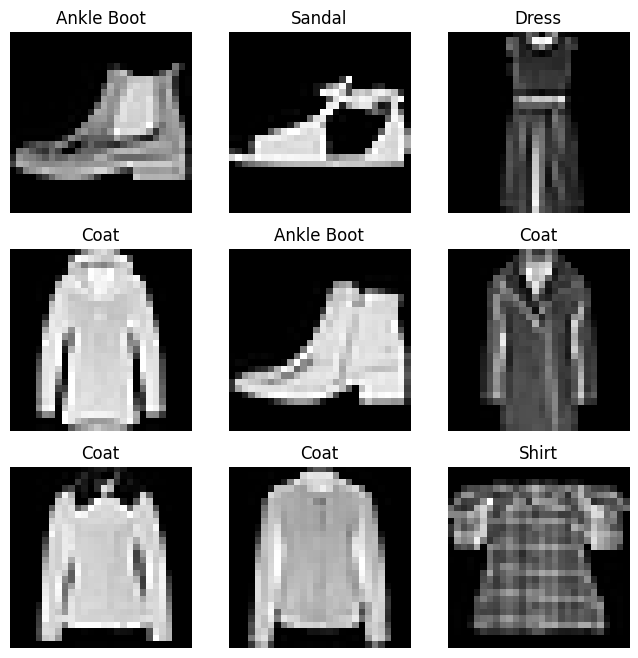
\includegraphics[width=0.7\textwidth]{figures/visualize.png}
    \caption{visualize the samples by matplotlib}
\end{figure}

\subsubsection{Dataloaders}
\textbf{} Dataloader is an iterable that abstracts the process of batching, shuffling, and loading the data. The dataset retrieves the dataset's features and labels one sample at a time. When we are training the model, we want reshuffle the data at every epoch to reduce model overfitting.

\begin{python}
    from torch.utils.data import DataLoader
    train_dataloader = DataLoader(training_data, batch_size=64, shuffle=True)
    test_dataloader = DataLoader(test_data, batch_size=64, shuffle=True)
\end{python}

\textbf{} When we loaded the data into the dataloader, we specify the batch size and shuffle. Each iteration of the dataloader will return a batch of train features and labels.

\begin{figure}[h]
    \centering
    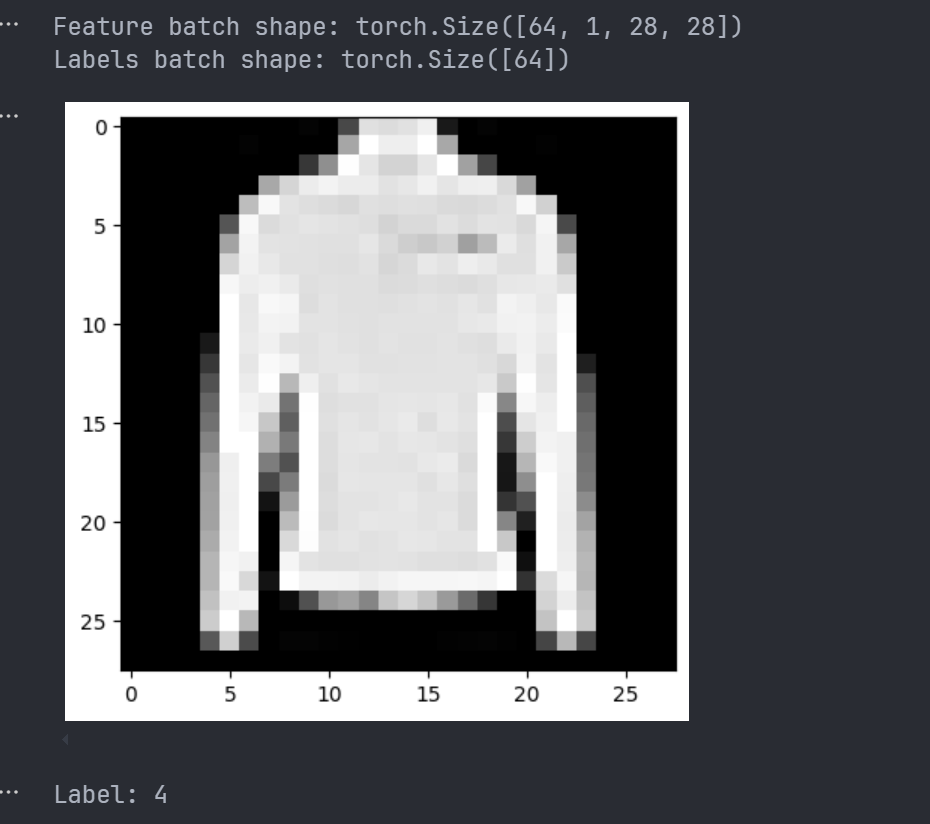
\includegraphics[width=0.7\textwidth]{figures/sample.png}
    \caption{Dataloader}
\end{figure}

\subsection{Transforms}
\textbf{} We always need to convert the data into tensors. When we load the data, we can use the transforms to convert the data into tensors. And we can also normalize and standardize the data.

\subsubsection{How to use transforms}
\begin{itemize}
\item \textbf{To Tensor:} Converts a PIL image or NumPy ndarray into a FloatTensor. And scales the image's pixel intensity values in the range [0., 1.]
\begin{python}
    my_transforms = transforms.Compose([transforms.ToTensor()])
\end{python}
\item \textbf{Lambda:} Applies a user-defined lambda function.
\begin{python}
    target_transform = Lambda(lambda y: torch.zeros(
        10, dtype=torch.float).scatter_(dim=0, index=torch.tensor(y), value=1))
\end{python}
\end{itemize}
\newpage

\subsection{Building Neural Network}
\textbf{} Neural networks are the core of both deep learning and machine learning.
\subsubsection{How to build a neural network}
\begin{itemize}
    \item \textbf{Perpare the data:} We need to prepare the data before we can use it to train the model.
    \item \textbf{Define a model structure} We define our neural network by subclassing nn.Module, and initialize the neural network layers. Every nn.Module subclass implements the operations on input data in the forward method.
    \item \textbf{Forward propagation:}  Calculate outputs through the network.
    \item \textbf{Loss calculation:} Calculate the loss using the model's output and the target. e.g. mean squared error loss (MSE) or cross-entropy loss. We can use the loss function from the torch.nn module. We always hope to minimize the loss.
    \item \textbf{Backward propagation:}  Update model parameters to minimize the loss by computing the gradient of the loss. Use optimization algorithms (such as gradient descent, Adam, RMSProp, etc.) for parameter updates.
\end{itemize}

\subsection{Automatic Differentiation}
\textbf{} When training neural networks, the most frequently used algorithm is back propagation. In this algorithm, model weights are adjusted according to the gradient of the loss function with respect to the given parameter.

\begin{figure}[h]
    \centering
    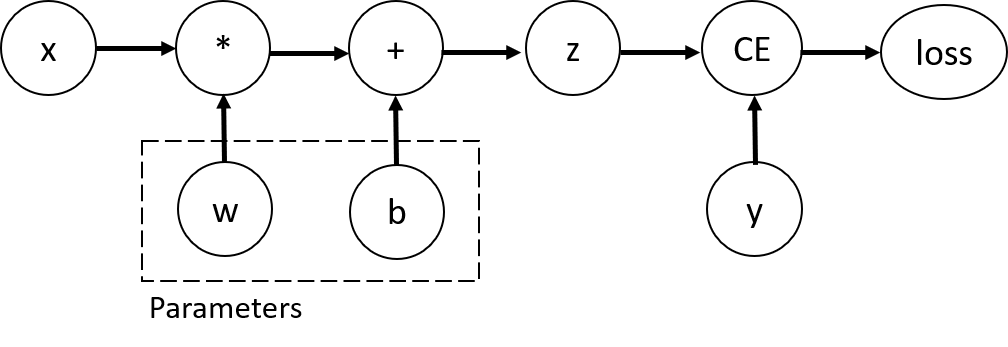
\includegraphics[width=0.5\textwidth]{figures/comp-graph.png}
    \caption{Computational Graph}
\end{figure}
\begin{equation}\label{eq:1}
    \begin{aligned}
        z = x \times w + b\\
    \end{aligned}
\end{equation}

\begin{equation}\label{eq:2}
    \begin{aligned}
        \text{loss} = CE(z,y)\\
    \end{aligned}
\end{equation}

If we in binary classification, CE can be Calculated as:
\begin{equation}\label{eq:3}
    \begin{aligned}
        CE = -y \times \log(\hat{y}) - (1-y) \times \log(1-\hat{y})\\
    \end{aligned}
\end{equation}

If we in multi-class classification, CE can be Calculated as:
\begin{equation}\label{eq:4}
    \begin{aligned}
        CE = -\sum_{i=1}^{n} y_i \times \log(\hat{y_i})\\
    \end{aligned}
\end{equation}

$y$ is binary indicator (0 or 1) if class label $i$ is the correct classification for sample $i$.\\

$\hat{y}$ is the predicted probability of class $i$.\\

\subsubsection{Computing Gradients}
\textbf{} We can compute the gradients of the loss with respect to the model parameters by loss.backward(). So that we need $ \frac{\partial loss}{\partial w}$ and $ \frac{\partial loss}{\partial b}$ under fixed values of $x$ and $y$.

\subsubsection{Disabling Gradient Tracking}
\textbf{} By default, all tensors are tracking their computational history and support gradient computation. However, we don't need to track the history for the weights and biases while training the model.
\begin{python}
    with torch.no_grad():
    z = torch.matmul(x, w)+b
\end{python}

\textbf{} When we want to mark some parameters in your neural network as frozen parameters or speed up computations(only doing forward propagation), we can turn off the gradient computation.

\subsection{Optimizers}
\textbf{}  Training a model is an iterative process; in each iteration the model makes a guess about the output, we use loss function to calculates the error in its guess  , collects the derivatives of the error with respect to its parameters, and optimizes these parameters using gradient descent.

\subsubsection{Hyperparameters}
\begin{itemize}
    \item \textbf{Learning Rate:} how much to update models parameters at each batch/epoch. 
    \item \textbf{Batch Size:} the number of data samples propagated through the network before the parameters are updated
    \item \textbf{Epochs:} the number times to iterate over the dataset
\end{itemize}

\subsubsection{Optimization Loop}
\begin{itemize}
    \item \textbf{Training loop:} iterate over the training dataset and try to converge to optimal parameters
    \item \textbf{Test loop:} iterate over the test dataset to check if model performance is improving
\end{itemize}

\subsubsection{Loss Function}
\textbf{}  Loss function measures the degree of dissimilarity of obtained result to the target value, and it is the loss function that we want to minimize during training. \\
e.g. Cross-Entropy Loss
\begin{python}
    loss_fn = nn.CrossEntropyLoss()
\end{python}

\subsubsection{Optimizer}
\textbf{} Optimization is the process of adjusting model parameters to reduce model error in each training step. Optimization algorithms define how this process is performed.\\

In the training loop, optimization happens in the following steps:
\begin{itemize}
    \item Call optimizer.zero\_grad() to reset the gradients of model parameters. Gradients by default add up; to prevent double-counting, we explicitly zero them at each iteration.
    \item Backpropagate the prediction loss with a call to loss.backward(). PyTorch deposits the gradients of the loss w.r.t. each parameter.
    \item Once we have our gradients, we call optimizer.step() to adjust the parameters by the gradients collected in the backward pass.
\end{itemize}

\subsection{Save and load model}

\subsubsection{Saving and loaing model weights}
\textbf{} PyTorch models store the learned parameters in an internal state dictionary, called state\_dict.
\begin{python}
    model = models.vgg16(weights='IMAGENET')
    torch.save(model.state_dict(), 'model.pth')
\end{python}

\textbf{} To load model weights we use the load\_state\_dict() method.
\begin{python}
    model = models.vgg166()
    model.load_state_dict(torch.load('model.pth'), weights_only=True)
    model.eval()
\end{python}

\subsubsection{Saving and loading the model with shapes}
\textbf{} When loading model weights, we needed to instantiate the model class first, because the class defines the structure of a network. We might want to save the structure of this class together with the model, in which case we can pass model to the saving function.
\begin{python}
    torch.save(model, 'model.pth')
\end{python}

\textbf{} We can then load the model like this:
\begin{python}
    model = torch.load('model.pth', weights_only=False)
\end{python}

\newpage 
\centering
Thank You for reading this article. 

\end{document}
